% Standalone 6.2 draft, not included in the official thesis main file.
\section{判别器设计与梯度优化机制}
\label{sec:ch06_discriminator_gradient}

共享向量场需要依据生成结果与Real观测的差异获得优化信号。触觉窗口既包含精确零值与非零值构成的激活支持，也包含正值响应的幅度变化。本文将两者作为判别输入，以分别保留支持模式和连续响应信息。它们均由同一触觉数组得到，并非相互独立的物理接触观测。对于生成窗口$Y$，判别器特征定义为
\begin{equation}
 \Phi(Y)=\left[\operatorname{vec}\!\left(\mathbf1[Y>0]\right),
 \operatorname{vec}\!\left(\frac{\log(1+Y)}{s_R}\right)\right],
 \label{eq:ch06_discriminator_features}
\end{equation}
其中$s_R=0.14118273556232452$由Real Train对数响应的总体标准差确定，不作均值中心化。两路各2848维，拼接为5696维，经192维Linear、LayerNorm和LeakyReLU，再经64维Linear、LeakyReLU及单输出层得到logit。LeakyReLU负半轴斜率为0.2，sigmoid将输出转为Real类别分数。

离散Mask在生成与判别两端分别出现，梯度问题也应分开讨论。令$a$为Real Decoder的Mask logit，其训练读出采用直通估计器（Straight-Through Estimator，STE）：
\begin{equation}
 m_{\rm hard}=\mathbf1[a\ge0],\qquad
 m_{\rm ST}=m_{\rm hard}+\sigma(a)-\operatorname{sg}(\sigma(a)),
 \label{eq:ch06_decoder_ste}
\end{equation}
其中$\operatorname{sg}$表示停止梯度，$\sigma$为sigmoid。前向仍以硬Mask乘Gamma混合幅值均值，反向借用sigmoid导数，解决的是Decoder内部从logit到输出的离散路径。生成触觉再次进入判别器时，后者重新计算$M_D=\mathbf1[Y>0]$；该比较在实现中不保留输入梯度，数学上阈值函数几乎处处导数为零。因此，Decoder的STE不会自动穿过判别器端的再次二值化，但连续幅值支路仍可提供梯度，不能将这一断点写成生成器完全无法训练。

为核查输入表示与梯度机制，设置表\ref{tab:ch06_discriminator_comparison}的三种配置。C组在判别输入端另加STE：
\begin{equation}
 \begin{aligned}
 q(Y)&=\sigma\!\left((Y-\epsilon)/\tau_m\right),\\
 M_{\rm ST}&=\mathbf1[Y>0]+q(Y)-\operatorname{sg}(q(Y)).
 \end{aligned}
 \label{eq:ch06_discriminator_ste}
\end{equation}
取$\epsilon=0$、$\tau_m=0.005002501420676708$，后者来自Real Train全部正值响应的中位数，不是搜索得到的阈值。$\tau_m$为代理温度，与积分坐标$\tau$不同。C组保持硬前向，仅改变反向；本对照未训练纯Soft-forward组。两处操作及梯度关系见图\ref{fig:ch06_mask_gradient_paths}。

\begin{figure}[htbp]
 \centering
 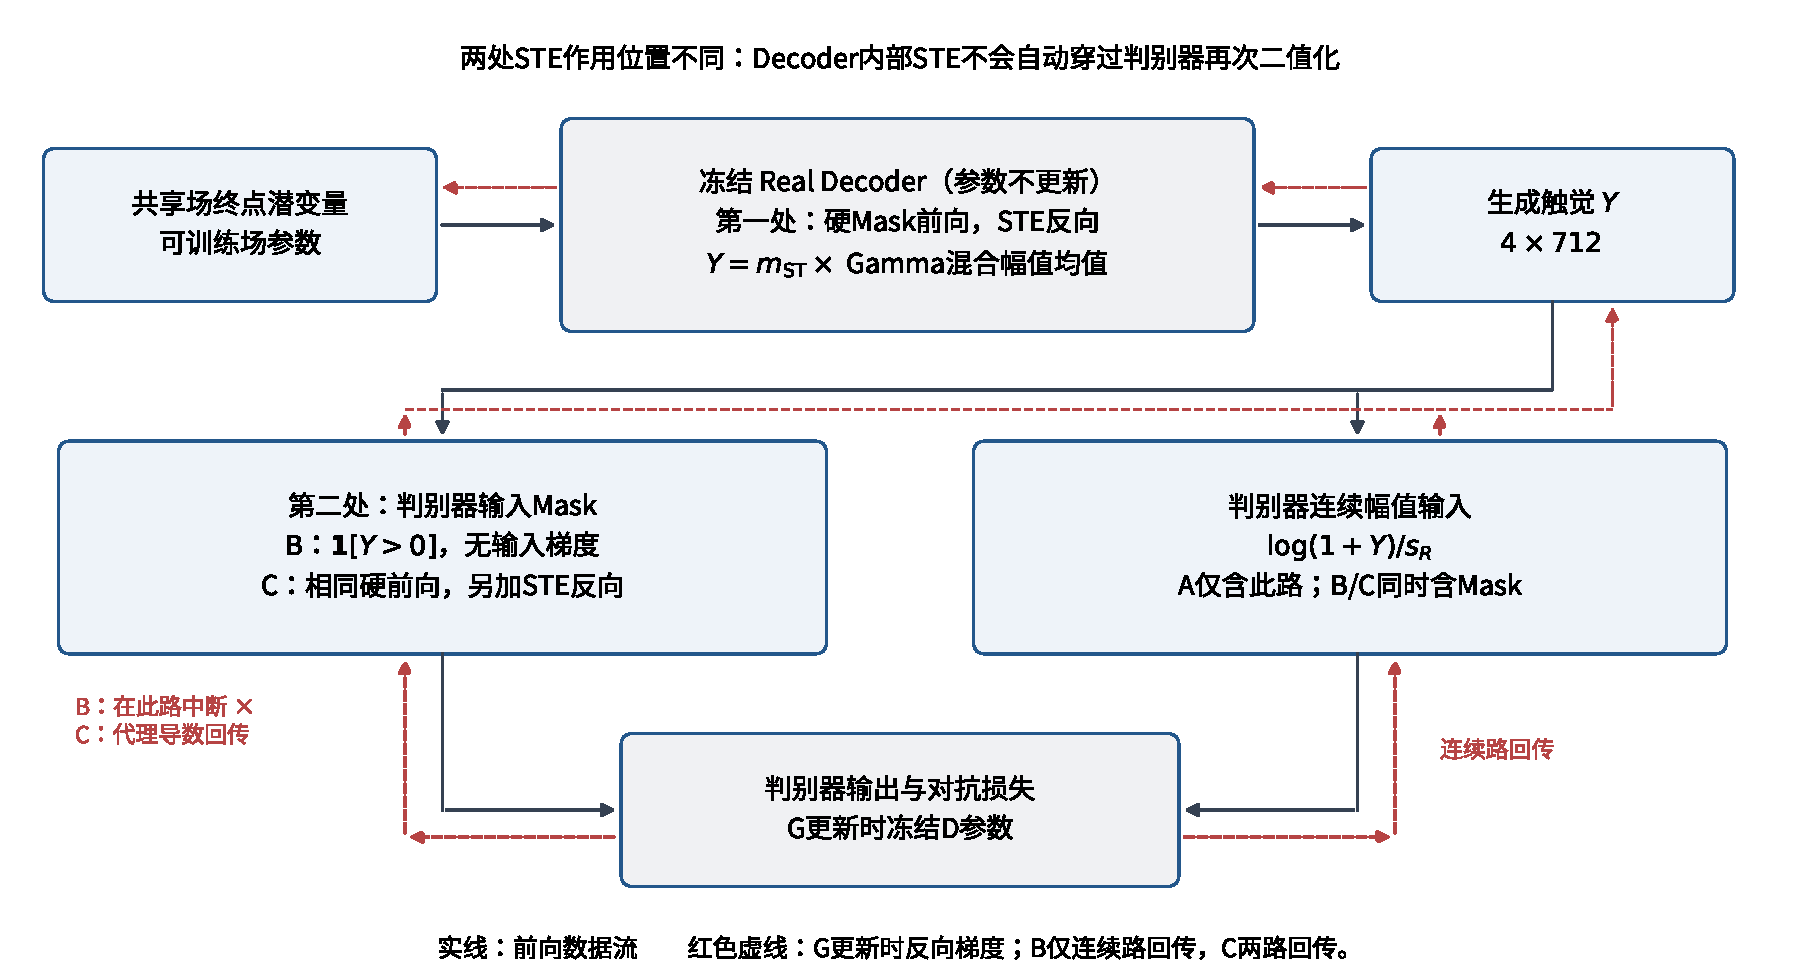
\includegraphics[width=\textwidth]{figures/ch06/mask_gradient_paths.pdf}
 \caption{Decoder与判别器输入端的两处Mask梯度路径。实线为前向，虚线为生成器更新时的反向；B组的判别Mask支路中断，C组以代理导数传递，连续支路保留。}
 \label{fig:ch06_mask_gradient_paths}
\end{figure}

\begin{table}[htbp]
 \centering\small
 \setlength{\tabcolsep}{4pt}
 \caption{判别器输入配置及原冻结C0联合结果}
 \label{tab:ch06_discriminator_comparison}
 \begin{tabular}{p{0.07\textwidth}p{0.20\textwidth}p{0.14\textwidth}p{0.27\textwidth}p{0.19\textwidth}}
 \hline
 组 & 输入维度 & 参数量 & Mask实现与初始化 & 联合通过数\\
 \hline
 A & 连续2848 & 559809 & 无显式Mask；复制幅值半列及共同层 & 1/0/0/0\\
 B & Mask与连续各2848 & 1106625 & 硬Mask；复用原运行 & 1/1/1/1\\
 C & Mask与连续各2848 & 1106625 & 硬前向STE反向；复制原D & 0/1/1/1\\
 \hline
 \end{tabular}
 \par\smallskip
 {\small 联合通过数依次对应$K=1,2,4,8$，各项分母均为11。}
\end{table}

三组生成器初始权重一致。A仅复制原D首层的幅值半列，其余共同层完全复制；C复制原D全部对应参数，A与C随后分别训练。B直接复用已有运行，并非第三次独立训练。A参数量较少，容量及有效正则路径不同，不能将其与B的差异纯归因于是否存在Mask。B与C容量相同，也仍受单Seed及固定训练配置限制。

训练采用两轮D预热及18轮G/D交替更新，Adam学习率$10^{-4}$、betas为$(0,0.99)$，梯度范数裁剪5。D以两类各半的批次平均BCE优化，Lazy R1每16步触发，$\gamma=0.1$，触发时系数为$\gamma\times16/2$。C在D更新及Real R1路径禁用Mask代理，避免额外改变这一正则机制；G更新时启用代理，冻结D参数但保留其对$Y$的梯度。生成器使用非饱和对抗项，并保留权重0.5295653698327406的Patch份额与相对帧差保持项、权重0.001的修正场约束，以及首个对抗轮从1衰减至第六轮0的同源教师项。场约束按Real Train后验均值的逐维标准差归一化，下限为0.1，只约束修正项，不含Translator基项；教师项比较同源输出按固定尺度归一化的对数响应差。各项沿用本次配置的窗口批次均值，不能套用后续组加权损失。A、C分别完成D1280步和G1152步，使用一致的窗口排列及步数调度，固定第20轮终点，不按C0结果选择权重。

梯度诊断采用前8个Natural Train窗口，以$K=8$展开，并逐支分离损失经判别特征到$Y$及向量场参数的导数；它衡量的是指定样本上的局部梯度，不是全部窗口的平均优化收益。既有记录显示，C组初始Mask支路回传至$Y$与向量场参数的梯度L2分别为4.618483、0.318322，终点为24.031830、27.183775，均有限。B组对应记录为零；A因不存在该支路，由诊断代码填零，不是测得一个硬Mask零导数。C因此建立了可达梯度，但代理导数并非硬阈值的真实导数，非零也不保证优化方向有利于完整重建。

原11个冻结C0实例仍沿用第五章的固定预处理及阈值。每个实例要求$\mathrm{BA}\in[0.45,0.55]$、$\mathrm{AUC}\in[0.475,0.525]$及域混淆指标$D_{\rm BA}\ge0.90$。表中所有候选的该指标专项均为11/11，但联合条件还要求AUC；BA与$D_{\rm BA}$门槛数学等价，不能重复当作独立证据。没有候选达到11/11联合通过；C修复梯度未解决完整迁移，B的部分通过也不能反推Mask梯度不重要。后续需要进一步检验多轮优化能否改善生成质量，以及判别器接受率能否充分反映这种改善。
